\documentclass[a4paper,12pt,oneside]{report}
\usepackage{natbib}         % Pour la bibliographie
\usepackage{url}            % Pour citer les adresses web
\usepackage[T1]{fontenc}    % Encodage des accents
\usepackage[utf8]{inputenc} % Lui aussi
\usepackage[french]{babel} % Pour la traduction française
\usepackage{numprint}       % Histoire que les chiffres soient bien
\usepackage{fancyhdr}

\usepackage{amsmath}        % La base pour les maths
\usepackage{mathrsfs}       % Quelques symboles supplémentaires
\usepackage{amssymb}        % encore des symboles.
\usepackage{amsfonts}       % Des fontes, eg pour \mathbb.
\usepackage{setspace}
\usepackage[svgnames]{xcolor} % De la couleur
\usepackage{geometry}       % Gérer correctement la taille

%%% Si jamais vous voulez changer de police: décommentez les trois
%\usepackage{tgpagella}
%\usepackage{tgadventor}
%\usepackage{inconsolata}
\usepackage{enumitem}
\usepackage{listings}
\usepackage{protobuf/lang}
\usepackage{protobuf/style}
\usepackage{graphicx} % inclusion des graphiques
\usepackage{wrapfig}  % Dessins dans le texte.

\usepackage{tikz}     % Un package pour les dessins (utilisé pour l'environnement {code})
\usepackage[framemethod=TikZ]{mdframed}
% Un environnement pour bien présenter le code informatique
\newenvironment{code}{%
\begin{mdframed}[linecolor=Green,innerrightmargin=30pt,innerleftmargin=30pt,
backgroundcolor=Black!5,
skipabove=10pt,skipbelow=10pt,roundcorner=5pt,
splitbottomskip=6pt,splittopskip=12pt]
}{%
\end{mdframed}
}


%\setmarginsrb{3 cm}{2.5 cm}{3 cm}{2.5 cm}{1 cm}{1.5 cm}{1 cm}{1.5 cm}
\graphicspath{{figures/}}

\title{Rapport de Stage Master 2}
\author{ABAK-KALI Nizar}
\date{\today}

\newcommand{\reporttitle}{Rapport de stage M2}
\newcommand{\reportauthora}{Nizar ABAK-KALI {11290569}} % Auteur
\newcommand{\reportsubject}{} % Sujet
\newcommand{\HRule}{\rule{\linewidth}{0.5mm}}
\setlength{\parskip}{1ex} % Espace entre les paragraphes
\makeatletter
\let\thetitle\@title
\let\theauthor\@author
\let\thedate\@date
\makeatother

\pagestyle{fancy}
\fancyhf{}
\rhead{\theauthor}
\lhead{\thetitle}
\cfoot{\thepage}
\lfoot{
  
\includegraphics [width=20mm]{figures/logop8.jpg}
  }
\rfoot{
  
\includegraphics [width=30mm]{figures/logo_Smile.png}
}
%\renewcommand{\footrulewidth}{1pt}


\begin{document}

%%%%%%%%%%%%%%%%%%%%%%%%%%%%%%%%%%%%%%%%%%%%%%%%%%%%%%%%%%%%%%%%%%%%%%%%%%%%%%%%%%%%%%%%
\begin{titlepage}

\begin{center}

\begin{minipage}[t]{0.48\textwidth}
  \begin{flushleft}
   
\includegraphics [width=30mm]{figures/logop8.jpg} \\[0.5cm]
    \begin{spacing}{1.5}
      %\textsc{Université Paris 8}
    \end{spacing}
  \end{flushleft}
\end{minipage}
\begin{minipage}[t]{0.48\textwidth}
  \begin{flushright}
    
\includegraphics [width=50mm]{figures/logo_Smile.png} \\[0.5cm]
    %\textsc{Neo-Robotix}
  \end{flushright}
\end{minipage} \\[1.5cm]

%\textsc{\Large \reportsubject}\\[0.5cm]
\HRule \\[0.4cm]
{\huge \bfseries \reporttitle}\\[0.4cm]
\HRule \\[1.5cm]

\begin{minipage}[b]{0.3\textwidth}
  \begin{flushleft} \large
    \emph{Auteurs :}\\
    \reportauthora\\
  \end{flushleft}
\end{minipage}
\begin{minipage}[b]{0.6\textwidth}
  \begin{flushright} \large
    \emph{Tuteur :} \\
    M.~Benoit \textsc{COURTY} \\
	M.~Jean Luc \textsc{COSSI} \\
   \end{flushright}
\end{minipage}

\vfill

{\large \today}

\end{center}

\end{titlepage}

\chapter*{Résumé du stage}
Ce stage s'est déroulé dans la société de services Smile et plus particulièrement le département Smile ECS, responsable de l'offre embarqué et IoT\footnote{IoT: Internet of Things ou objets connectés}. Ainsi, mon stage s'est d'abord déroulé sous la tutelle de Pierre Lamot, expert en traitement d'images et streaming chez Smile ECS, puis sous celle de Fabien Dutuit, expert traitement de signal.
\\
Au cours de ce stage, j'ai eu l'opportunité de travailler sur une grande variété de technologies et ainsi d'avoir la chance de pouvoir engranger un maximum de connaissances et d'expériences dans le monde de l'embarqué que je compte utiliser plus tard.
\newline
\newline
Ce stage se découpe en deux phases. Un premier concentré sur l'étude du protocole MPEG-TS ainsi que de son implémentation dans Gstreamer\footnote{\ref{gstreamer}} puis de l'écriture d'un patch décri plus tard dans le rapport, permettant le multiplexage de données non typé dans un flux vidéo. Puis dans un second temps, mon stage c'est plus concentré sur le projet SisselBox\footnote{\ref{sisselbox}}, où je devais dans un premier temps mettre à jour le système de provisionnement, puis implémenter une application afin de tester mon patch.

%%%%%%%%%%%%%%%%%%%%%%%%%%%%%%%%%%%%%%%%%%%%%%%%%%%%%%%%%%%%%%%%%%%%%%%%%%%%%%%%%%%%%%%%%
\tableofcontents
%%%%%%%%%%%%%%%%%%%%%%%%%%%%%%%%%%%%%%%%%%%%%%%%%%%%%%%%%%%%%%%%%%%%%%%%%%%%%%%%%%%%%%%%%
\listoffigures
\pagebreak
%%%%%%%%%%%%%%%%%%%%%%%%%%%%%%%%%%%%%%%%%%%%%%%%%%%%%%%%%%%%%%%%%%%%%%%%%%%%%%%%%%%%%%%%%
\chapter*{Remerciements}
  A l'issue de ce stage, je souhaite remercier l'équipe technique de Smile ECS\footnote{Embdeed Computer Science} de m'avoir accordé une place dans leur département d'embarquer et de m'avoir permis d'effectuer mon stage de fin d'étude au sein d'une équipe compétente et conviviale. Je remercie également M. Pierre Lamot, expert technique ECS, pour m'avoir soutenu et motivé pendant le stage, et tant apporté.Je souhaite également remercier M. Fabien Dutuit, expert technique ECS, pour m'avoir aidé dans les difficultés que j'ai pu rencontrer, et pour ces encouragement . Je souhaite remercier également toute l'équipe de Smile ECS qui m'a supporté durant ces 6 mois, mais qui m'a avant tout apporté énormément aussi bien sûr le plan humain que technique.


\chapter*{Introduction}

Dans le cadre de mon master en informatique embarqué à l'université paris 8, il est
nécessaire d’effectuer un stage de fin d’étude d’une durée de 6 mois en entreprise.
Après avoir prospecté plusieurs offres de stage et avoir effectué plusieurs entretient,
mon choix s’est finalement porté vers la société Smile et plus particulierement le département
embarqué.
J’ai donc rejoint l'équipe de Smile ECS, filiale spécialisée dans l’infor-matique
embarquée et le traitement des images à destination des industriels.
Mon stage s’est donc déroulé du 20 février au 18 aout 2017 au sein de Smile ECS,
à Asnieres.



\chapter{Présentation de l'entreprise}

\section{Smile}

Fondé en 1991, Smile est devenu dès 1995 un acteur du web réputé, maîtrisant l’architecture, les techniques et les outils qui permettent de construire les plus grandes plateformes de l’Internet.
Depuis 2001, Smile est intégrateur de solutions open source, c'est-à-dire que le cœur de métier de Smile est la construction de systèmes d’informations et de plateformes web intégrant les meilleures solutions open source du marché.
Smile mène une forte action de veille afin d’identifier les solutions open sources les plus matures et les plus pérennes, qui apporteront un réel bénéfice de compétitivité pour les entreprises. Smile met à disposition un échantillon de cette expertise au travers de livres blancs, librement diffusés, qui sont devenus des références dans leurs domaines.
Premier intégrateur spécialisé sur les solutions open source, Smile a été choisi à de nombreuses reprises par les plus grandes entreprises et administrations pour déployer ces solutions dans le cadre de projets stratégiques.
Autour du cœur de métier qu’est l’ingénierie, Smile propose une palette de services étendus, qui lui permet de prendre en charge un projet dans sa globalité : consulting en amont et en accompagnement des projets, agence interactive intervenant tant en création et web design où’en conseils éditoriaux, stratégiques et e-marketing, tierce-maintenance applicative (TMA), formation, support et maintien en conditions opérationnelles, et enfin hébergement et exploitation.
Smile possède également un rayonnement international grâce à ses dix-sept agences réparties dans 9 pays.

\begin{figure}[!h]
  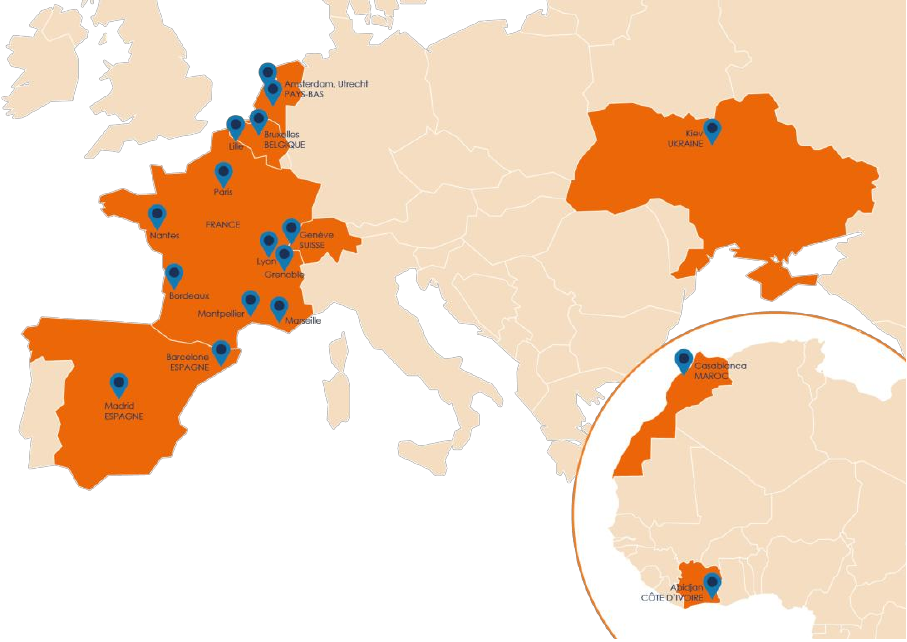
\includegraphics[scale=0.7]{carte_smile}
  \caption{\label{smile_map} Agences Smile}
\end{figure}

Smile organise également une veille technologique importante sur l’open source, avec la rédaction de nombreux livres blancs par les différents consultants sur des sujets variés allant des solutions web d’e-commerce, en passant par les middlewares et finissant par l’embarqué. Il existe actuellement une vingtaine de livres blancs, renouvelés tous les 2-3 ans pour inclure les nouveautés des différents techniques.Dès 2001, Smile commence à construire son expertise des solutions open source : un choix d’avenir que beaucoup de ses concurrents n’osent pas alors entreprendre.À partir de 2004, les grandes entreprises adoptent de plus en plus souvent les solutions open source. Smile occupe une position solide de leader sur ce marché qui décolle, élargissant progressivement son offre vers de nouveaux domaines – CMS, Portails, e-Commerce;Décisionnel, Infrastructure, ERP - et créant des services associés : agence média, tierce maintenance, exploitation, système.  En 2007, Smile affiche plus de 50\% de croissance et inaugure trois nouvelles agences à Lyon, Nantes et Bordeaux.En 2008, Smile compte plus de 270 collaborateurs et poursuit sa croissance en se développant à l'international, notamment à Kiev en Ukraine.En 2009, Smile compte 320 collaborateurs dans le monde et poursuit son extension internationale. En juin 2009, Smile intègre Cometa Technologies S.L., basée à Barcelone et compte alors 8 agences dans le monde.En 2011, Smile regroupe 500 collaborateurs et ouvre ses agences à Bruxelles, Utrecht etAmsterdam.
En 2013, Smile compte 700 collaborateurs et 17 agences.
2014 est une année importante pour Smile, avec plus de 20\% de croissance sur ces cinq
dernières années et près de 700 collaborateurs dans le monde. Au fil de ces années, Smile est
devenu un acteur incontournable de l’open source, leader en France et en Europe.
En 2015, Smile annonce être en négociations exclusives avec la société Open Wide en vue
d’un rapprochement. Ceci afin d'élargir son offre et renforcer son leadership.


\section{Smile ECS}
Smile ECS, ex-Openwide est une société spécialisée dans le domaine de l'open source, racheté par Smile. J'ai décidé d'intégrer cette entreprise pour mon projet de fin d'études à l'université Paris 8 afin d'approfondir mes connaissances dans le domaine du logiciel libre, et celui de l'embarqué. Les techniques Open source devenant de plus en plus prédominants dans le paysage informatique moderne, intégrer une société spécialisée dans cette technique était une façon pour moi de donner un cap sur l'orientation de ma carrière professionnelle.Ce rapport explicitera mon travail durant ce stage de fin d'études, qui a duré six mois, dont le sujet a été d'améliorer le système de transmission des données, afin de pouvoir transmettre un flux vidéo, de caméras de sécurité, avec des métadonnées calculées depuis ce flux (exemple: positions des visages détectés). Puis dans un second temps, récupérer ce flux afin de le stocker pour un visionnage ultérieur.Après une explication du cadre du stage, j'essaierai de développer les techniques utilisés lors de ce stage.
\newpage
\section{Présentation du sujet}
Mon sujet s'inscrit dans un projet developpé en interne, le projet SisellBox. Ansi,
je vais présenter dans un premier temps le projet, puis dans un second temps
expliquer ou je m'inscrit dans le projet et qu'est ce que j'y apporte.

\subsection{Le projet SisellBox}
  \subsubsection{ça fait quoi}
  \subsubsection{pour qui}
  \subsubsection{Architecture du projet (Schéma + commentaire)}
  $\rightarrow$ schema general de la sBox
  \begin{itemize}
    \item Sbox Streamer
    \item Sbox Recorder
  \end{itemize}

\subsection{La problématique posé}
\begin{itemize}
  \item Etude de Gstreamer
  \item Etude du protocole MPEG-TS
  \item Transmission de flux vidéo + métadonnée
  \item patch du plugin Gstreamer mpegtsmux afin de  multipler les donnes
  \item patch du plugin de Gstreamer mpegtsdemux afin demultplexer les données pour le stockage
  \item afficher les metadonnée sur une une interface a
\end{itemize}

\newpage
\chapter{Présentation de l'environnement de travail}
Dans le cadre de se stage j'ai eu l'occasion de travailler une plusieurs technologie, beaucoup d'entre-elles m'était inconnue. Ainsi , je vais explicité les différentes technologie sur lesquelles j'ai travailler.
\section{Configuration}
Ubuntu 16.04, python v2, Vala v 0.3,

\section{Gstreamer}
\label{gstreamer}



GStreamer est un framework multimédia sous licence libre publié pour la première fois le 31 octobre 1999. Il est écrit en C est initialement pensé pour être un solution concurrente à QuickTime et Direct Show sur GNU/Linux. Aujourd'hui, GStreamer est disponible pour de nombreux systèmes d'exploitations (GNU/Linux, Solaris, BSD, Android, OS X, iOS, Windows, OS/400). De plus, des bindings existent pour utiliser GStreamer dans une multitude de langages de programmation en plus du C (C++, Java, Python, Vala etc..)
\begin{figure}[!h]
  \centering
  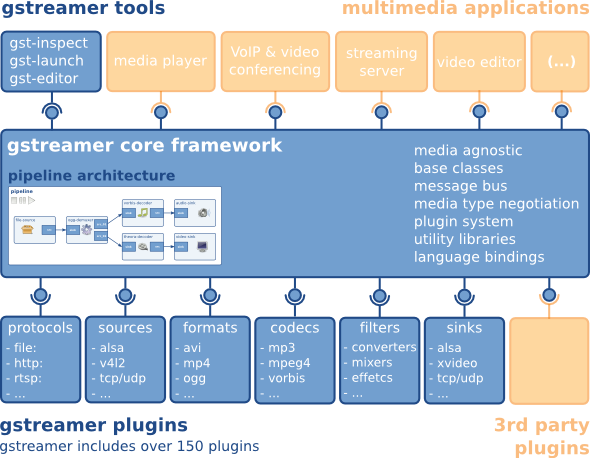
\includegraphics[scale=0.7]{figures/gstreamer-overview}
  \caption{schéma de l'architecture de Gstreamer}
\end{figure}



\subsection{Principes techniques}
GStreamer est basé sur un système de pipeline. Différents éléments sont connectés entre eux par des tuyaux (pipe). Chaque élément possède des « pad » servant à les connecter aux autres. Ces pads peuvent être soit des entrées (sink) soit des sorties (source).
Exemple de pipeline GStreamer :
Cette pipeline lit un fichier *.ogg, en sépare les pistes et décode sa piste audio et la décode pour ensuite la jouer.

\begin{figure}[!h]
  \centering
  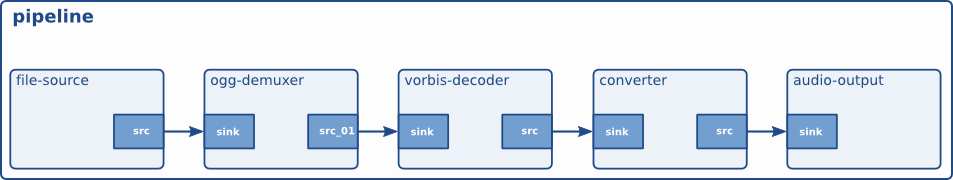
\includegraphics[scale=0.5]{figures/pipeline_ogg}
  \caption{Une pipeline gstreamer pour lire un fichier .ogg puis decode en vorbis}
\end{figure}

Une autre notion importante de GStreamer est celle de « capabilities » (capacités) ou «caps». Il s'agit d'une liste de formats et propriétés d’un flux qu'un élément peut accepter sur un pad. Par exemple, un élément acceptant uniquement un format vidéo/x-raw au framerate 24/1 (24 images par secondes) ne pourra pas recevoir d'autre flux (format ou framerate différent). Ainsi les caps peuvent imposer un format, une résolution, un framerate, etc. Ce sont eux qui sont utilisés par GStreamer pour négocier la connexion entre deux éléments et choisir le type de flux qui sera utilisé (si les caps sont compatibles pour au moins un type de flux, sinon la négociation échoue).

\begin{figure}[!h]
  \centering
  
\includegraphics[scale=0.9]{figures/caps_negociation}
  \caption{pipeline avec négociation de caps}
\end{figure}

\subsection{Présentation des composants Gstreamer}
Le framework Gstreamer offre plusieurs types d'éléments, ou "plugins", afin d'effectuer des taches différentes. Gstreamer fourni plus de 200 plugins différent. Ainsi ils permettent :
\begin{itemize}[label=$\bullet$]
 \item la manipulation d’objet multimédia
 \item gestions des entrées audio/vidéo (caméra/flux réseau)
 \item gestion des protocoles réseaux
 \item gestion des filtres
 \item gestion des sorties
\end{itemize}

Lors de ce stage, j'ai particulierement travailler avec deux types d'élément, les multipléxeurs (ou "muxers") et les démultipléxeurs (ou " demuxers"). Les muxers sont de élement "N-to-1" qui prennent N flux en entrée puis les "entrelace" en un seul. Particulierement utiles lorsque l'on voudra muxer le flux vidéo avec la métadonnée.
Les démuxers font l'exact inverse, ainsi, ils prennent un flux "entrelacé" puis en fourni N.



\subsubsection{3.2.1.2 Débogage}
GStreamer possède des outils de débogage très utiles qui m'ont servis tout au long du stage. Le premier est GST\_DEBUG. Il s'agit d'une variable d’environnement qui peut être initialisé avec une valeur de 1 à 9 permettant d'afficher plus ou moins d'informations sur le déroulement des actions initiées par GStreamer.
L'autre outils est un générateur de fichier *.dot permettant de générer une représentation graphique de la pipeline. Cela permet de vérifier que la pipeline obtenue par le programme est bien celle souhaitée lors de la conception et permet repérer simplement et rapidement certaines erreurs


\section{OpenCV}
Le projet contient des briques algorithmiques fonctionnant grâce à la bibliothèque OpenCV. OpenCV (pour Open Computer Vision) est une bibliothèque graphique libre, initialement développée par Intel, spécialisée dans le traitement d'images en temps réel. La société de robotique Willow Garage et la société ItSeez se sont succédé au support de cette bibliothèque, Depuis 2016 et le rachat de ItSeez par Intel, le support est de nouveau assuré par Intel.


\section{Protobuf et Grpc}

\subsection{Protobuf}
Protobuf ou "Protocol Buffers" sont un mécanisme flexible, efficace et automatisé pour sérialiser des données structurées - pensez XML, mais plus petit, plus rapide et plus simple. Vous définissez comment vous souhaitez que vos données soient structurées une fois, vous pouvez utiliser un code source généré spécialement pour écrire et lire facilement vos données structurées vers et à partir d'une variété de flux de données et en utilisant diverses langues. Vous pouvez même mettre à jour votre structure de données sans rompre les programmes déployés qui sont compilés par rapport au format.

\begin{lstlisting}[language=protobuf2,style=protobuf , frame=single,caption=modèle pour la structure d'un message,label=proto1]

 message Person {
  required string name = 1;
  required int32 id = 2;
  optional string email = 3;

  enum PhoneType {
    MOBILE = 0;
    HOME = 1;
    WORK = 2;
  }

  message PhoneNumber {
    required string number = 1;
    optional PhoneType type = 2 [default = HOME];
  }

  repeated PhoneNumber phone = 4;
}

\end{lstlisting}
C'est à l'aide de cet technologie que nous formattons les métadonnées générer par les algorithmes de traitement d'images afin de les "muxer" avec le flux vidéo.


\section{Outils de provisionnement}

\subsection{Vagrant}
Vagrant est un outil de création et de gestion d'environnements de machines virtuelles.
Grâce à un flux de travail facile à utiliser et à l'automatisation, lVagrant réduit le temps d'installation de l'environnement de développement, augmente la parité de production .
\subsection{Ansible}



\newpage
\section{Travail effectué}

\subsection{Etude de MPEG-TS}
         $->$ Pourquoi ? \\
         $->$ qu'est ce que c'est\\
         $->$ modification des plugins pour le mux/demux\\

\subsection{Projet SisselBox}
         $->$ Mis à jour du système de provisionnement\\
         $->$ Etude de l'existant\\
             - Sisell elements\\
             - sboxstreamer\\
         $->$ Création d'un application Test : MPEGTS[video+metadata]\\
              - pipeline
              - probleme de perte de flux par perte de synchro

\newpage
\chapter{Conclusion}

(à peu près 1 page)

­ ??? (conclusion du stage)

­ Quelques chose de personnel : ton sentiment, ce que tu en as tiré, ??

­ Ouverture vers la suite :

\newpage
\chapter*{Bibliographie}

\begin{description} 

\item [Sources des plugins mpegtsmux et mpegtsdemux] \url{https://github.com/GStreamer/gst-plugins-bad/tree/master/gst/mpegtsmux} et \url{https://github.com/GStreamer/gst-plugins-bad/tree/master/gst/mpegtsdemux}

\item [How To Install and Use PostgreSQL on Ubuntu 16.04 DigitalOcean] \url{https://www.digitalocean.com/community/tutorials/how-to-install-and-use-postgresql-on-ubuntu-16-04} . 
\item [GStreamer-1.8.1 rtsp server and client on ubuntu Telecom R \& D] \url{https://telecom.altanai.com/2016/05/20/gstreamer-1-8-1-rtsp-server-and-client-on-ubuntu/} . 
\item [gstreamer - Plugins: "ugly" and "bad" - Ask Ubuntu] \url{https://askubuntu.com/questions/468875/plugins-ugly-and-bad} . 
\item [grpc] \url{http://www.grpc.io/docs/quickstart/cpp.html} . 
\item [grpc] \url{http://www.grpc.io/docs/quickstart/python.html} . 
\item [Projects · Dashboard · GitLab] \url{https://gitlab.openwide.fr/} . 
\item [gst-plugins-base/gst-libs at master · GStreamer/gst-plugins-base · GitHub] \url{https://github.com/GStreamer/gst-plugins-base/tree/master/gst-libs} . 
\item [Installing OpenCV 2.4.9 in Ubuntu 14.04 LTS – Sebastian Montabone] \url{http://www.samontab.com/web/2014/06/installing-opencv-2-4-9-in-ubuntu-14-04-lts/} . 
\item [Installing OpenCV on Debian Linux | Indranil's world] \url{https://indranilsinharoy.com/2012/11/01/installing-opencv-on-linux/} . 
\item [grpc/INSTALL.md at master · grpc/grpc · GitHub] \url{https://github.com/grpc/grpc/blob/master/INSTALL.md} . 
\item [Gstreamer basic real time streaming tutorial | Einar Sundgren] \url{http://www.einarsundgren.se/gstreamer-basic-real-time-streaming-tutorial/} . 
\item [GStreamer Debugging - RidgeRun Developer Connection] \url{https://developer.ridgerun.com/wiki/index.php/GStreamer_Debugging#Use_standard_GStreamer_debug_output_with_filter} . 
\item [manual.pdf] \url{https://gstreamer.freedesktop.org/data/doc/gstreamer/head/manual/manual.pdf} . 
\item [open-wide / sisellbox-ng · GitLab] \url{https://gitlab.openwide.fr/open-wide/sisellbox-ng} . 
\item [Accueil - Smile Intranet] \url{https://intranet.smile.fr/portal/fr/web/guest/home} . 
\item [Webmail - BlueMind] \url{https://bluemind.smile.fr/webmail/?_task=mail&_mbox=INBOX&_refresh=1} . 
\item [Vim as a Python IDE | Unlogic] \url{http://unlogic.co.uk/2013/02/08/vim-as-a-python-ide/} . 
\item [Real Time Streaming Protocol - Wikipedia] \url{https://en.wikipedia.org/wiki/Real_Time_Streaming_Protocol} . 
\item [toto.html] \url{file:///home/niaba/Documents/sisellbox-ng/doc/architecture/toto.html} . 
\item [Troubleshooting GStreamer] \url{https://gstreamer.freedesktop.org/documentation/frequently-asked-questions/troubleshooting.html} . 
\item [Gstreamer cheat sheet - MyLabWiki] \url{http://wiki.oz9aec.net/index.php/Gstreamer_Cheat_Sheet} . 
\item [pygst-tutorial.pdf] \url{https://brettviren.github.io/pygst-tutorial-org/pygst-tutorial.pdf} . 
\item [Instantiable classed types: objects: GObject Reference Manual] \url{https://developer.gnome.org/gobject/stable/gtype-instantiable-classed.html} . 
\item [GObject Reference Manual: GObject Reference Manual] \url{https://developer.gnome.org/gobject/stable/} . 
\item [Mpeg TS helper library: GStreamer Bad Plugins 1.0 Library Reference Manual] \url{https://gstreamer.freedesktop.org/data/doc/gstreamer/head/gst-plugins-bad-libs/html/mpegts.html} . 
\item [gst-plugins-bad/gst-libs/gst/mpegts at master · GStreamer/gst-plugins-bad] \url{https://github.com/GStreamer/gst-plugins-bad/tree/master/gst-libs/gst/mpegts} . 
\item [Diapo : ces bricolages de génie qui donnent envie d'acheter un Raspberry Pi] \url{http://www.tomshardware.fr/articles/raspberry-pi-bestof-bricolage-hack,1-63056.html} . 
\item [MPEG transport stream - Wikipedia] \url{https://en.wikipedia.org/wiki/MPEG_transport_stream#PCR} . 
\item [Novacut/GStreamer1.0 - Ubuntu Wiki] \url{https://wiki.ubuntu.com/Novacut/GStreamer1.0} . 
\item [rubenrua/GstreamerCodeSnippets: Gstreamer Code Snippets in C, Python and Shell (gst-launch).] \url{https://github.com/rubenrua/GstreamerCodeSnippets} . 
\item [Adding Properties] \url{https://gstreamer.freedesktop.org/documentation/plugin-development/basics/args.html} . 
\item [Example GStreamer Pipelines - IGEP Community Wiki] \url{http://labs.isee.biz/index.php/Example_GStreamer_Pipelines} . 
\item [Base MPEG-TS descriptors: GStreamer Bad Plugins 1.0 Library Reference Manual] \url{https://gstreamer.freedesktop.org/data/doc/gstreamer/head/gst-plugins-bad-libs/html/gst-plugins-bad-libs-Base-MPEG-TS-descriptors.html} . 
\item [Creating special element types] \url{https://gstreamer.freedesktop.org/documentation/plugin-development/element-types/index.html} . 
\item [GStreamer and in-band metadata - RidgeRun Developer Connection] \url{https://developer.ridgerun.com/wiki/index.php/GStreamer_and_in-band_metadata} . 
\item [Novacut/GStreamer1.0 - Ubuntu Wiki] \url{https://wiki.ubuntu.com/Novacut/GStreamer1.0#audio.2Fx-raw.2C_video.2Fx-raw} . 
\item [cerbero-docs/start.md at master · centricular/cerbero-docs] \url{https://github.com/centricular/cerbero-docs/blob/master/start.md} . 
\item [centricular/cerbero: GStreamer's Cerbero forked to add Meson and MSVC support] \url{https://github.com/centricular/cerbero} . 
\item [GstPlugin: GStreamer 1.0 Core Reference Manual] \url{https://gstreamer.freedesktop.org/data/doc/gstreamer/head/gstreamer/html/GstPlugin.html} . 
\item [YBlog - Learn Vim Progressively] \url{http://yannesposito.com/Scratch/en/blog/Learn-Vim-Progressively/} . 
\item [The Basics of Writing a Plugin] \url{https://gstreamer.freedesktop.org/documentation/plugin-development/basics/index.html} . 
\item [Things to check when writing an element] \url{https://gstreamer.freedesktop.org/documentation/plugin-development/appendix/checklist-element.html} . 
\item [Shared Libraries] \url{http://tldp.org/HOWTO/Program-Library-HOWTO/shared-libraries.html} . 
\item [Install Qt 5 on Ubuntu - Qt Wiki] \url{https://wiki.qt.io/Install_Qt_5_on_Ubuntu} . 
\item [Vim Awesome] \url{http://vimawesome.com/} . 
\item [Base MPEG-TS descriptors: GStreamer Bad Plugins 1.0 Library Reference Manual] \url{https://gstreamer.freedesktop.org/data/doc/gstreamer/head/gst-plugins-bad-libs/html/gst-plugins-bad-libs-Base-MPEG-TS-descriptors.html#GstMpegtsDescriptor-struct} . 
\item [Base MPEG-TS sections: GStreamer Bad Plugins 1.0 Library Reference Manual] \url{https://gstreamer.freedesktop.org/data/doc/gstreamer/head/gst-plugins-bad-libs/html/gst-plugins-bad-libs-Base-MPEG-TS-sections.html} . 
\item [MPEG-2 TS Overview] \url{http://cmm.khu.ac.kr/korean/files/02.mpeg2ts1_es_pes_ps_ts_psi.pdf} . 
\item [Packetized elementary stream - Wikipedia] \url{https://en.wikipedia.org/wiki/Packetized_elementary_stream} . 
\item [GStreamer-devel - Gstreamer-1.0 blacklisted entries] \url{http://gstreamer-devel.966125.n4.nabble.com/Gstreamer-1-0-blacklisted-entries-td4671087.html} . 
\item [DevDocs — Offline] \url{https://devdocs.io/offline} . 
\item [Example GStreamer Pipelines - Texas Instruments Wiki] \url{http://processors.wiki.ti.com/index.php/Example_GStreamer_Pipelines} . 
\item [GStreamer Debugging - RidgeRun Developer Connection] \url{https://developer.ridgerun.com/wiki/index.php/GStreamer_Debugging} . 
\item [gst-launch-1.0] \url{https://gstreamer.freedesktop.org/documentation/tools/gst-launch.html#environment-variables} . 
\item [Basic tutorial 11: Debugging tools] \url{https://gstreamer.freedesktop.org/documentation/tutorials/basic/debugging-tools.html#the-debug-log} . 
\item [Sisselbox | Trello] \url{https://trello.com/b/2O788DTs/sisselbox} . 
\item [GStreamer Typefinding and Dynamic Pipelines - Part 2 · pyVision] \url{https://pi19404.github.io/pyVision//2014/12/17/21/} . 
\item [OpenVPN < Systeme/ConfigPostes < Foswiki] \url{https://wiki.smile.fr/view/Systeme/ConfigPostes/OpenVPN#Installation_client_Linux_40Debian_45_Ubuntu_41} . 
\item [Good patching practice] \url{http://en.tldp.org/HOWTO/Software-Release-Practice-HOWTO/patching.html} . 
\item [7 Patch Command Examples to Apply Diff Patch Files in Linux] \url{http://www.thegeekstuff.com/2014/12/patch-command-examples} .
\item [Developer Guide Protocol Buffers] \url{https://developers.google.com/protocol-buffers/docs/overview#what-are-protocol-buffers} .

\end{description}

\end{document}
